\section{Background}
\label{sec:background}

\subsubsection{OAuth2.0}
\begin{enumerate}[label=(\Alph*)]
\item {Overview}\\
OAuth is an authorization protocol where clients are granted access to the user's data at the resource provider. So OAuth exposes the resources and services at the resource provider with permission from the user so that, for a duration of time, the client has limited access to the resources on the user's behalf. So when you let an app sign in with Google or LinkedIn etc., and when it asks the user for permission, this app will have access to your email id, contacts etc. You provide the permission to access your resources hosted by the resource provider.
\item {Protocol flow}\\
Any client that wants to implement the OAuth flow has to first to register itself as an application at the resource provider. It gets assigned a unique Client ID and secret which is kept confidential. The general workflow for obtaining the access token is the following:
\begin{itemize}
\item The client redirects the user to the  authorization page  at the resource provider with client ID, redirect URI, scope, response type and state. The response type has to be set to "code" in this step. The redirect URI should match the one specified in the application registration. 
\item The resource server prompts the user for its credentials and also permission to allow/deny access to the client
\item Once the user authorizes the client, the authorization code is sent to the redirect URI specified in step 1. 
\item The client then sends a POST request with the authorization code, client ID and secret, grant type set to "authorization code" and redirect URI to exchange the code for the access token. This redirect URI should ideally match the one used when requesting for the code. This token can then be used to make API calls to the resource server. 
\end{itemize}
	\begin{figure}[t]
    		\centering
   		 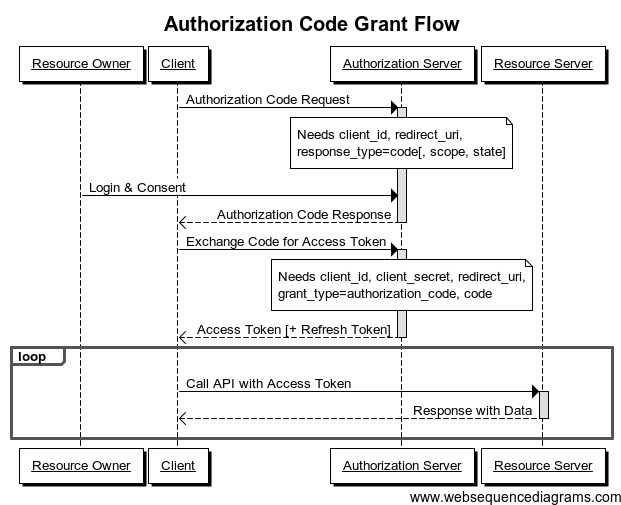
\includegraphics[width=\columnwidth]{figures/auth_code_flow.png}.
    		\caption{OAuth2.0 protocol flow}
    		\label{fig:flow}
	\end{figure} ~\\
The authorization code flow can be seen in Figure 1. 
OAuth2.0 uses two different credentials :\\
\textit{Access token:}
It represents access provided by the user. This token can be used by the client to make API calls to the resources at the provider. For example, a client can access the files in Google drive by using the access token obtained during authorization. It eventually expires but it can also last for a long time. 

\textit{Code:}
The code is used to get an access token. This request as mentioned should include the client secret. The code is not long lived and expires almost immediately. 
\end{enumerate}

\subsection{Threat Model}
\label{sec:threat}
\textbf{Attackers:} The attackers can be any individual or organization that intends to hijack the user's account resources and perform malicious activities on his behalf as well as passively obtaining user information by logging him in through the attacker's account. The capabilities of such an attacker need not be tremendous. He/she can be a simple weak attacker who is capable of luring the victim to a malicious application. A good understanding of the OAuth2.0 code flow can enable the attacker to tweak parts of the code to obtain information he/she requires. 

